

\chapter{Revisiting Sampling}

\section{Introduction}

In this chapter we revisit \autoref{chap:intro_sampling_dft}, mainly the sampling part, and dive into practical and application.\\

\uti{Revisiting Sampling:} \todo{Revisiting Sampling}

\begin{itemize}

\item \textit{This chapter need also some refactoring later, since it contain allot ot concepts, related to various topics}

\item \textit{Topics are from what I am seeing:}

	\begin{itemize}
	\item \textit{Filter desing,\autoref{sec:practical_filtering}}
	
	\item \textit{Communication aspect, \autoref{sec:appli}}
	\end{itemize}



\end{itemize}




\newpage

\section{Practical Sampling and Reconstruction}
\label{Sec:Sampling:Practical_Sampling and_Reconstruction}

Impulse sampling is one way we can get samples from the signal. Another way we can get samples is known as zero-order-hold (ZOH) as shown in \autoref{fig:Sampling:sampling_zoh}.

\begin{figure}[h]
\centering
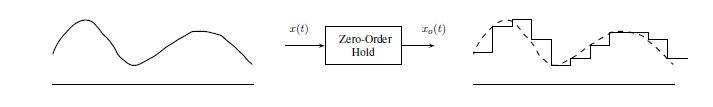
\includegraphics[width = 0.7\textwidth, frame]{Figures/Sampling/sampling_zoh}
\caption{Sampling using ZOH}
\label{fig:Sampling:sampling_zoh}
\end{figure}


It is named zero-order-hold because this filter grab a value of the signal, and then hold this value till it grab the next value. So the ZOH filter returns a stair case like signal, where each value of the signal is held till the next sampling time occurred.\\

Mathematical modeling of the ZOH is shown in \autoref{fig:Sampling:zoh_math}. 


\begin{figure}[h]
\centering
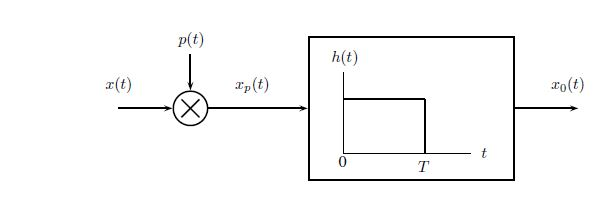
\includegraphics[width = 0.7\textwidth, frame]{Figures/Sampling/zoh_math}
\caption{Mathematical modeling of the ZOH}
\label{fig:Sampling:zoh_math}
\end{figure}


We have our continuous time signal $x(t)$ multiplied by an infinite train of pulse $p(t)$, then we obtain like before $x_p(t)$ which is equal to $x_{\delta}(t)$, then we do some low pass filtering using a pulse of width $T$. Amplitude spectrum of ZOH is shown in \autoref{fig:Sampling:zoh_amp_spectrum}. Recall that when we work in the digital domain, the only thing we care about is between $\pm \, \omega_s$.

\begin{figure}[h]
\centering
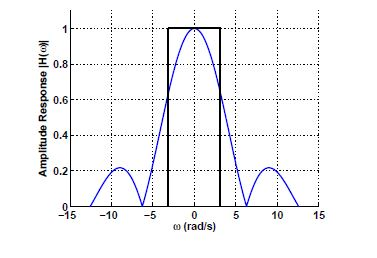
\includegraphics[width = 0.7\textwidth, frame]{Figures/Sampling/zoh_amp_spectrum}
\caption{Amplitude Spectrum of ZOH: boxed region is between $\pm \, \omega_s$}
\label{fig:Sampling:zoh_amp_spectrum}
\end{figure}


\underline{Spectrum of the Signal Compared to Impulse sampling of \autoref{fig:Sampling:impulse_sampling_spectrum_1}:}\\

Spectrum of the signal $x(t)$ using ZOH is shown in \autoref{fig:Sampling:zoh_output_spectrum}.

\begin{figure}[h]
\centering
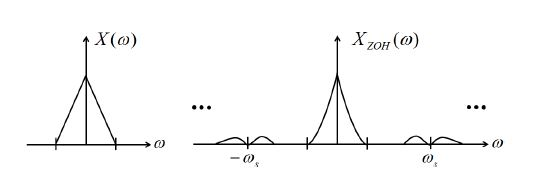
\includegraphics[width = 0.7\textwidth, frame]{Figures/Sampling/zoh_output_spectrum}
\caption{Output of ZOH in the frequency domain}
\label{fig:Sampling:zoh_output_spectrum}
\end{figure}

\begin{itemize}

\item In impulse sampling (see \autoref{fig:Sampling:impulse_sampling_spectrum_1}), the spectrum was the same (with the scale factor $\displaystyle\frac{1}{T_s}$), along with the replicate at multiple of $\omega_s$.


\item In ZOH, these replicate are attenuated due to the low pass nature of the ZOH, which is a good thing since we don't want these images.

\item However, the original spectrum is getting distorted, and this distortion is controlled by the time sampling we choose to get our values. 

\end{itemize}

\subsection{Mathematical Formulation for ZOH}

Ideal sampling followed by ideal bandlimited interpolation can't by done practically:

\begin{itemize}

\item Generating dirac pulses is very difficult

\item In reconstruction, the value of $\hat{y}(t)$ at a value of $t$ not multiple of $T_s$ is obtained by infinite sum of weighted sinc function

\item Ideal filters are also can't be made

\end{itemize}


ZOH is the practical way to grab a signal, which is done by taking a sample of the signal, and holding this value during the sampling interval.\\

Let's denote the rectangular pulse we are using by $h(t)$ denoted by:

\begin{equation}
h(t)\, = \, \begin{cases}
1 \quad 0 \, \leq \, t \, \leq \, T_s \\
0 \quad \text{otherwise}
\end{cases}
\end{equation}

The $x_{\text{zoh}}$ can be written as:

\begin{equation}
x_{\text{zoh}} \, = \, \displaystyle\sum\limits_{n \, = \, -\infty}^{\infty} x(n) h\left(	t \, - \, n\,T_s \right)
\label{Eq:Sampling:Zoh_eq_1}
\end{equation}

Recall that we can obtained a shifted version of a signal by convolving this signal with a dirac function so equation (\ref{Eq:Sampling:Zoh_eq_1}) can be further formulated:

\begin{equation}
\begin{array}{rcl}
x_{\text{zoh}} \, &=& \, \displaystyle\sum\limits_{n \, = \, -\infty}^{\infty} x(n) \, h\left(	t \, - \, n\,T_s \right) \\ \\		
&=& \, \displaystyle\sum\limits_{n \, = \, -\infty}^{\infty} x(n) \, \times \, \left[ \, \delta \left(	t \, - \, n\,T_s \right) \, * \, h(t) \, \right] \\ 
\end{array}
\label{Eq:Sampling:Zoh_eq_2}
\end{equation}


Manipulating the parenthesis of equation (\ref{Eq:Sampling:Zoh_eq_2}):

\begin{equation}
\begin{array}{rcl}
x_{\text{zoh}} \, &=& \, \displaystyle\sum\limits_{n \, = \, -\infty}^{\infty} x(n) \, h\left(	t \, - \, n\,T_s \right) \\ \\		
&=& \, \displaystyle\sum\limits_{n \, = \, -\infty}^{\infty} x(n) \, \times \, \left[ \, \delta \left(	t \, - \, n\,T_s \right) \, * \, h(t) \, \right] \\ \\
&=& \, \displaystyle\sum\limits_{n \, = \, -\infty}^{\infty} \left[\, x(n) \, \times  \, \delta \left(	t \, - \, n\,T_s \right) \, \right] \, * \, h(t)   \\ \\
&=& \,  x_{\delta}(t) \, * h(t)
\end{array}
\label{Eq:Sampling:Zoh_eq_3}
\end{equation}


Taking the Fourier transform of (\ref{Eq:Sampling:Zoh_eq_3}) we get:

\begin{equation}
\begin{array}{rcl}
X_{\text{zoh}}(\omega_c) \, &=& \, X_{\delta}(\omega_c) \, \times \, H(\omega_c) \\ \\
			 &=& \, \displaystyle\frac{1}{T_s} \, \displaystyle\sum\limits_{n  =  -\infty}^{\infty} X_a \left( \, \omega_c \, - \,  n \, \omega_s \right) \, \times \, 2 \, \text{exp}\left( \, -j \, \displaystyle\frac{\omega_c \, T_s}{2} \, \right) \, \times \, \text{sinc}\left(\, \displaystyle\frac{\omega_c \, T_s}{2} \,\right) 
\end{array}
\end{equation}

Since the rectangular pulse of \autoref{fig:Sampling:zoh_math} is not centered at 0, and it is shifted by $\displaystyle\frac{T_s}{2}$, we obtain a phase shift of $ 2 \, \text{exp}\left( \, -j \, \displaystyle\frac{\omega_c \, T_s}{2} \, \right)$ multiplying the sinc function.


\subsection{Reconstruction for ZOH}


Time delay by the factor of  $\displaystyle\frac{T_s}{2}$ can't be corrected, we have to deal with it. However, the distortion in original spectrum and the replication can be fixed.\\

\underline{Key notes in designing anti-imaging filter:}

\begin{itemize}

\item the key difficulty is in the transition band, where we need to suddenly pass to 0 in the stop band

\item This can be easily achieved if we have a high transition band, which implies that $\omega_s >> \,$ bandwidth signal

\item We later get back to this point when covering oversampling and undersampling, and how they can make the design of the anti-imaging filter less or more expensive.

\end{itemize}


\newpage
\section{Applications}
\label{sec:appli}

Sampling theorems let us replace a continuous time signal with a discrete set of numbers, so all we have to do now is to process these discrete numbers.\\ 

In this section we will look to some application of sampling, like how we can use the sample values to change the characteristic of a pulse.

A pulse can have different characteristics, like amplitude, width, position,$\cdots$. We start first by the following type of pulse modulation: PAM, PWM, PPM, and then treat PCM separately because it is the most sophisticated one among them.


\subsection{PAM, PWM and PPM}

\autoref{fig:Sampling:pulse_modulation} shows different type of pulse modulation

\begin{figure}[h]
\centering
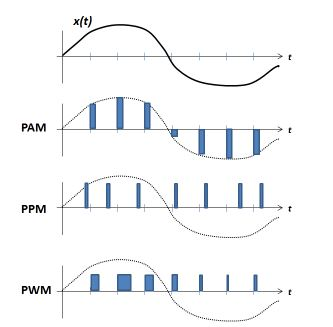
\includegraphics[width = 0.7\textwidth, frame]{Figures/Sampling/pulse_modulation}
\caption{Pulse Modulation}
\label{fig:Sampling:pulse_modulation}
\end{figure}

\begin{itemize}

\item In PAM: the more the sample value is higher, the amplitude of the pulse is higher

	\begin{itemize}
	\item The more the value is negative, same of the amplitude of the pulse
	\end{itemize}

\item In PPM, the width and amplitude of the pulses are all the same. However, the position of the pulse change

	\begin{itemize}
	\item If the value is more positive, the pulse become more early before the sample value
	
	\item If the value is negative, the pulse will be delayed and come after the sample value
	
	\item So we can now about sample value depending if the pulse arrive more early (more positive) or more delayed (more negative)
	\end{itemize}

\end{itemize}


\subsection{Quantization and A/D Process}

Before getting into PCM, we need to do learn some concepts whihc are prerequist to PCM. Let's start by some definitions:

\begin{itemize}

\item \tbi{Digital Signal:} discrete time signal and also discrete amplitude values

	\begin{itemize}
	\item Another definition of digital signal is that can be any continuous time signal which represents a stream of bits, like in PCM
\end{itemize}


\item \tbi{Quantization:} the process of rounding continuous valued amplitudes to a set of discrete amplitudes	

\begin{itemize}
\item Continuous-Time Signals Are Converted To Digital Signals By
Sampling and Quantizing (A/D converters do this)
\end{itemize} 

\item L-ary signal: A digital signal that can take on L different values

	\begin{itemize}
	\item Advantages of digital signal: resiliant to noise, use
of repeaters, error correction scheme more easy on digital signal (as opposite to continuous time signal which can take any value),
	\end{itemize}

\end{itemize}

\underline{Example of Quantization:}\\


\begin{figure}[h]
\centering
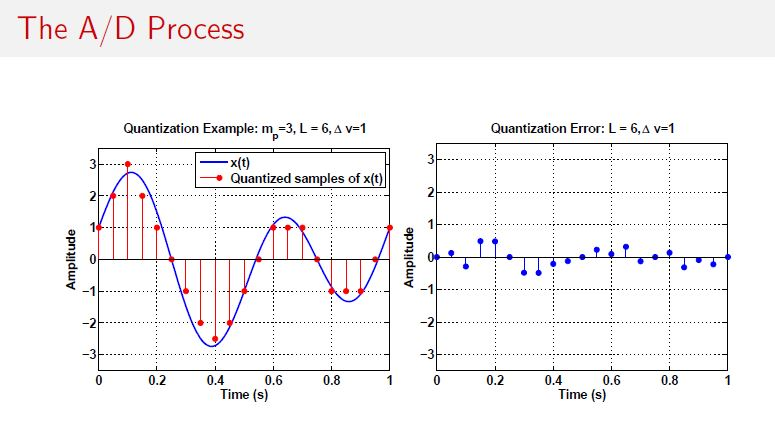
\includegraphics[width = 0.7\textwidth, frame]{Figures/Sampling/quantizaiton_example}
\caption{Quantization Example}
\label{fig:Sampling:quantizaiton_example}
\end{figure}


\begin{itemize}

\item In A/D process, first we sample the signal then we round up the value to a defined level

\item The parameters of the quantization (rounding) are:

	\begin{enumerate}
	\item The number of levels $L$: here we have 6 levels
	
	\item The step size between each level $\delta v$
	
	\item The peak value of the signal $m_p$
	\end{enumerate}


\newpage
\item Now \tbi{rounding introduce errors}, known here as \tbi{quantization error}

	\begin{itemize}
	\item If we want to decrease the quantization error, we need to increase the number of levels $L$ as \autoref{fig:Sampling:quantizaiton_example_2}
	
	\item However we need to allocate more bits to represents all of these levels (trade off)
	
	
	\begin{figure}[h]
\centering
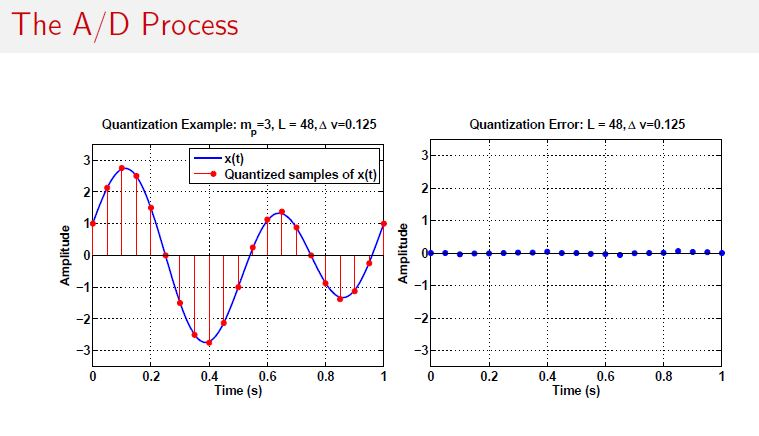
\includegraphics[width = 0.7\textwidth, frame]{Figures/Sampling/quantizaiton_example_2}
\caption{Increasing number of levels $L$ to decrease quantization error}
\label{fig:Sampling:quantizaiton_example_2}
\end{figure}
	
	\end{itemize}

\end{itemize}


\subsection{PCM}

PCM is a modulation scheme where we represent a stream of bits (after sampling and quantizing) into a sequence of pulses. An example is shown in \autoref{fig:Sampling:pcm_modulation}


\begin{figure}[h]
\centering
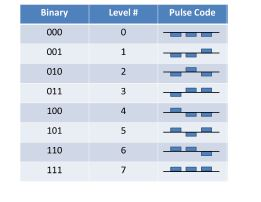
\includegraphics[width = 0.7\textwidth, frame]{Figures/Sampling/pcm_modulation}
\caption{PCM modulation using $L \, = \, 8$ levels}
\label{fig:Sampling:pcm_modulation}
\end{figure}

\begin{itemize}

\item After finishing the A/D process, we do mapping to these discrete numbers into a stream of bits


\item The the stream of bits is represented using pulses

	\begin{itemize}
	\item 1 using an positive pulse and 0 using a negative pulse
	\end{itemize}

\end{itemize}

\newpage
\section{Practical Digital Filtering and Oversampling}
\label{sec:practical_filtering}

\begin{figure}[h]
\centering
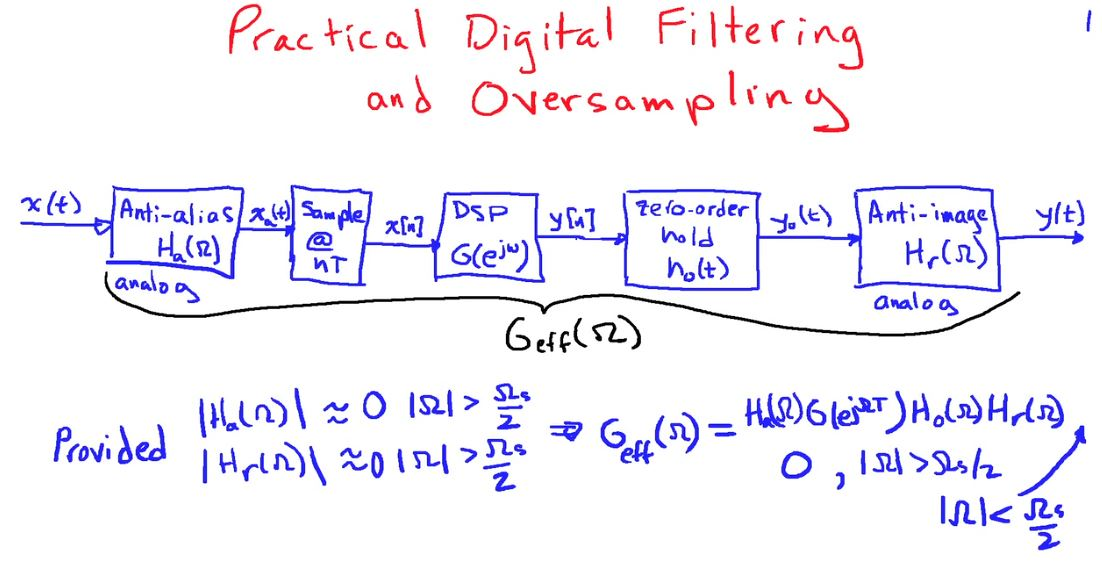
\includegraphics[width = 0.7\textwidth, frame]{Figures/Sampling/overall_sampling_reconstruction}
\caption{Overall Sampling and Reconstruction process}
\label{fig:Sampling:overall_sampling_reconstruction}
\end{figure}

\begin{itemize}

\item The DSP system is in the discrete frequency domain $\omega_d$

\end{itemize}

We can replace the whole system by a equivalent analog filter called $G_{\text{eq}}(\omega_c)$ where the transfer function is the multiplication of each transfer function block.

\subsection{Building Analog filters}


There are 2 filters presented in \autoref{fig:Sampling:overall_sampling_reconstruction} which are both \tbi{analog}: the anti-aliasing filter $H_{\text{ant}}(\omega_c)$ which cut high frequency to \tbi{prevent folding} and anti-imaging filter $H_{\text{ant-img}}(\omega_c)$ to \tbi{smooth the signal} after the ZOH operation.\\




\begin{itemize}

\item  For the anitliasing filter: if $\displaystyle\frac{\omega_s}{2}$ is close to the bandwidth of the signal $\omega_{\text{signal}}$, this means that the \tbi{transition band} of the filter is \tbi{very narrow} and that's \tbi{hard to implement in analog filters}.


\item For the anti-imaging filter: in the pass-band of the filter, we need to implement the inverse of the sinc to compensate the distortion made by the main lobe of the ZOH filter.

We need to make $\omega_s$ larger compared to the bandwidth of the signal so we don't have narrow band transition and the pass band 

\end{itemize}


So in summary, we need a high sampling rate. But in implementation, this comes at the cost excessive memory storage, because if my sampling rate is high, I have more data to process in a 1s, which means we need more memory for the storage.\\

So there is a trade-off between a high sampling rate and the memory needed for storage.

As a solution, we will change the sampling rate in the system of \autoref{fig:Sampling:overall_sampling_reconstruction}:

\begin{itemize}

\item Decrease the sampling rate after the ADC process, right before the discrete processing

\item Increase the sampling rate right before the ZOH

\end{itemize}


The new process including upsampling and downsampling is shown in \autoref{fig:Sampling:up_down_sampling}. 


\begin{figure}[h]
\centering
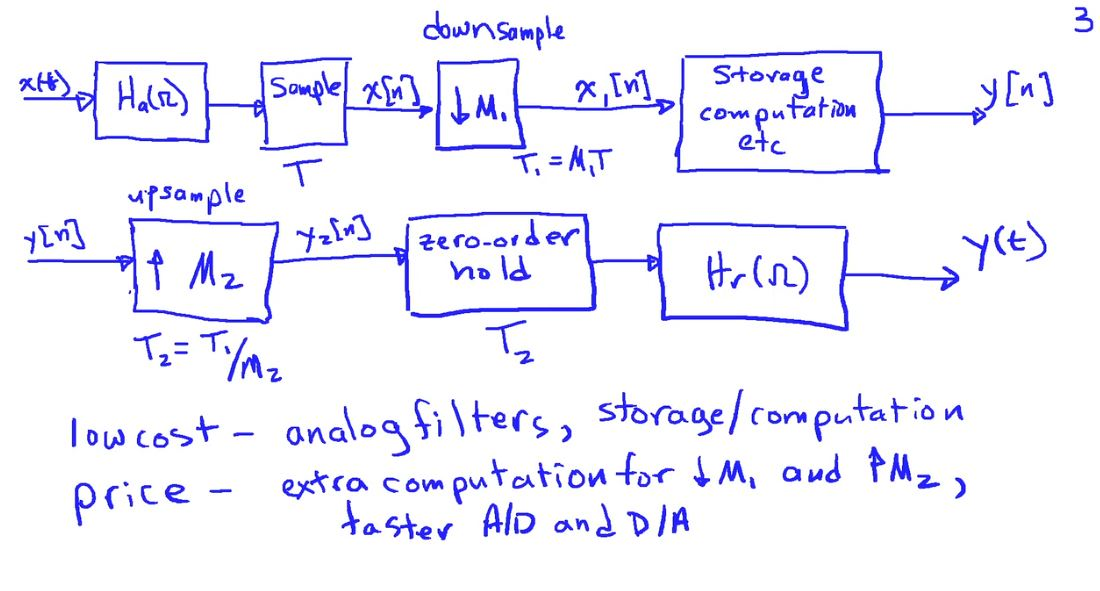
\includegraphics[width = 0.7\textwidth, frame]{Figures/Sampling/up_down_sampling}
\caption{Upsampling and downsampling for lower cost analog filters}
\label{fig:Sampling:up_down_sampling}
\end{figure}


\begin{itemize}

\item There are many efficient numerical methods to implement the up and down sampling operations

\item The price we pay in these discrete operations is worthy and make the design of the analog filters (anti-aliasing and anti-imaging) less expensive

\end{itemize}

\newpage
\subsection{Example of Oversampling}


Given are shown in \autoref{fig:Sampling:example_oversampling}.

\begin{figure}[h]
\centering
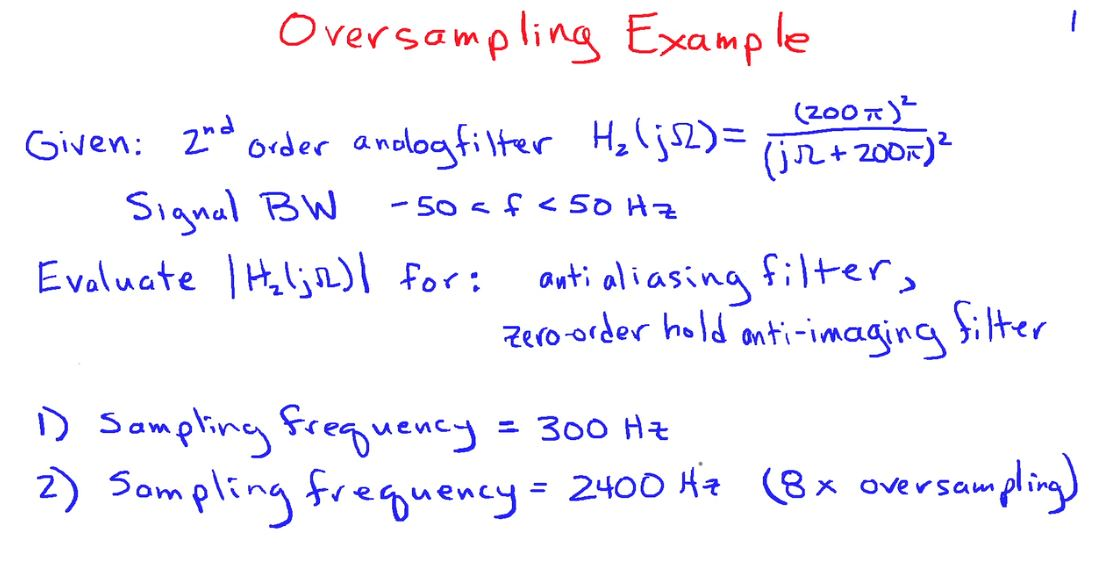
\includegraphics[width = 0.7\textwidth, frame]{Figures/Sampling/example_oversampling}
\caption{Given Example for oversampling}
\label{fig:Sampling:example_oversampling}
\end{figure}


The goal of this exercise is to show how oversampling can serve the analog filters (anti-aliasing and anti-imaging).


\begin{itemize}

\item The filter is an analog $\mathrm{2}^\mathrm{nd}$ order filter

\item The signal bandwidth is 50 Hz.

\item 2 sampling rate which both satisfy the Nyquist rate will be tested

\end{itemize}

\underline{Solution:}\\

\begin{enumerate}

\item For the anti-aliasing filter: \\

\begin{figure}[h]
\centering
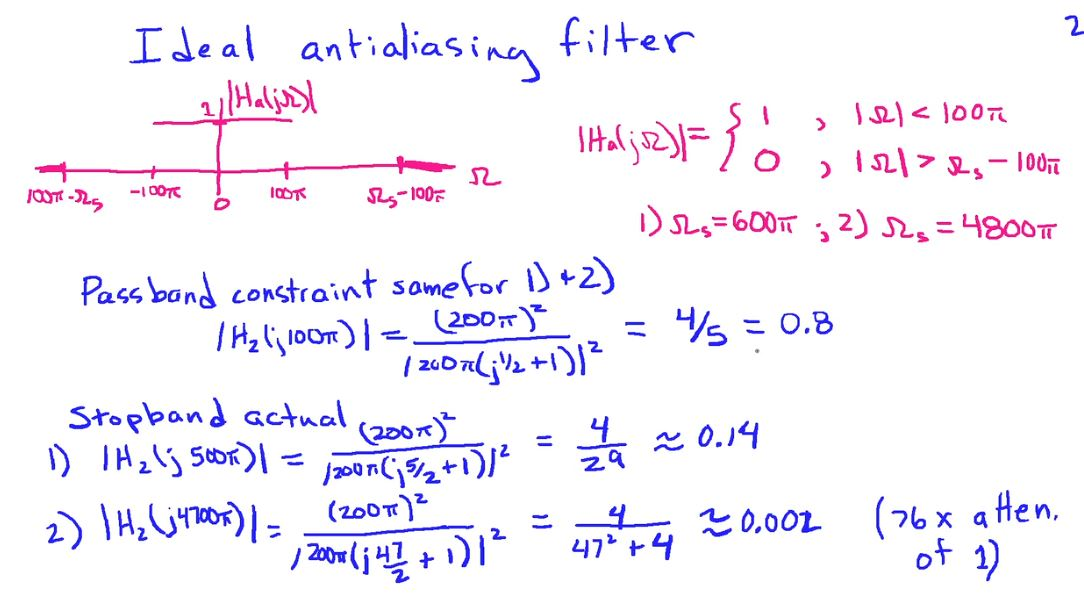
\includegraphics[width = 0.7\textwidth, frame]{Figures/Sampling/example_oversampling_sol_1}
\caption{Anti-aliasing filter solution}
\label{fig:Sampling:example_oversampling_sol_1}
\end{figure}

	\begin{itemize}
	
	\item The ideal anti-aliasing filter has an amplitude response of 1 in the pass-band and 0 in the stop band.
	
	\item Then we plug the computation for both $\omega_s$ and see the results	
	
	\begin{itemize}
	\item in the pass-band, the filtering is independent from $\omega_s$ so for both sampling rate, we have $ \mid H_{\text{ant-alias}}(\omega_c) \mid \, = \, 0.8$
	
	\item In the stop band we have the difference because the stop-band depend on $\omega_s$
	
	\end{itemize}
	
	\end{itemize}


 \item For the anti-imaging filter:

\begin{figure}[h]
\centering
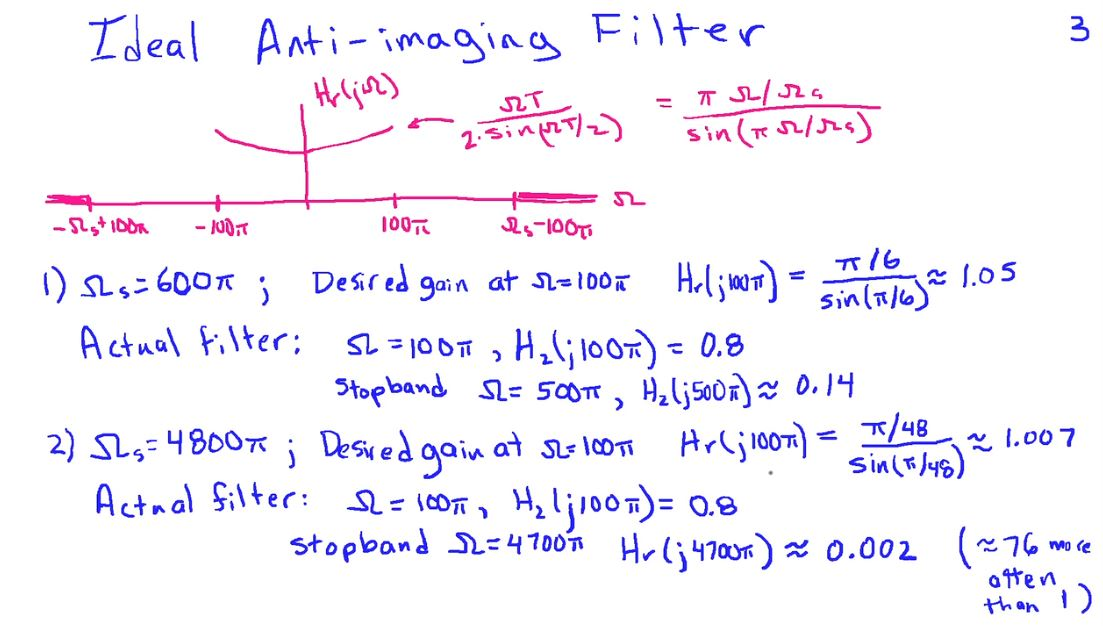
\includegraphics[width = 0.7\textwidth, frame]{Figures/Sampling/example_oversampling_sol_anti_imaging}
\caption{Anti-imaging filter solution}
\label{fig:Sampling:example_oversampling_sol_anti_imaging}
\end{figure}

\begin{itemize}

\item The ideal anti-imaging filter has the inverse of the sinc function as a frequency response


\item Also, the benefit is in the stop band, where oversampling is giving us more attenuation then the $ F_s \, = \,300 $ Hz

\end{itemize}

\end{enumerate}

\newpage
\subsection{Oversampling in D/A}

\autoref{fig:Sampling:oversampling_benefits} shows the D/A process.

\begin{figure}[h]
\centering
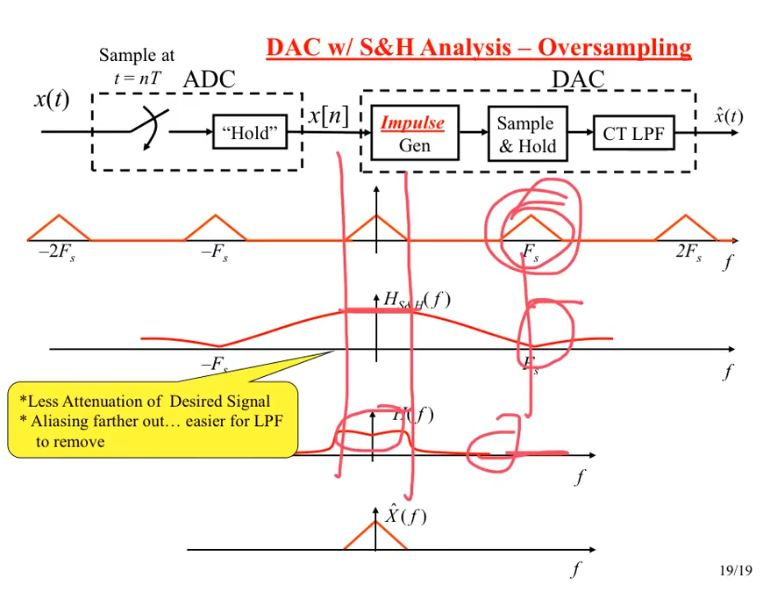
\includegraphics[width = 0.7\textwidth, frame]{Figures/Sampling/oversampling_benefits}
\caption{Over sampling Benefits}
\label{fig:Sampling:oversampling_benefits}
\end{figure}

Oversampling have several benefits:

\begin{itemize}

\item Make the frequency response of the ZOH system more flat in the pass band

\item Easier transition band design for the smoothing filter

\end{itemize}


\newpage
\section{Quantization and A/D Process}

In this section, we study quantization and its error.

\underline{Reminder:}\\

\begin{itemize}

\item \tbi{Digital Signal:} discrete time signal and also discrete amplitude values

	\begin{itemize}
	\item Another definition of digital signal is that can be any continuous time signal which represents a stream of bits, like in PCM
\end{itemize}


\item \tbi{Quantization:} the process of rounding continuous valued amplitudes to a set of discrete amplitudes	

\begin{itemize}
\item Continuous-Time Signals Are Converted To Digital Signals By
Sampling and Quantizing (A/D converters do this)
\end{itemize} 

\item L-ary signal: A digital signal that can take on L different values

	\begin{itemize}
	\item Advantages of digital signal: resiliant to noise, use
of repeaters, error correction scheme more easy on digital signal (as opposite to continuous time signal which can take any value),
	\end{itemize}

\end{itemize}

\underline{Example of Quantization:}\\


\begin{figure}[h]
\centering
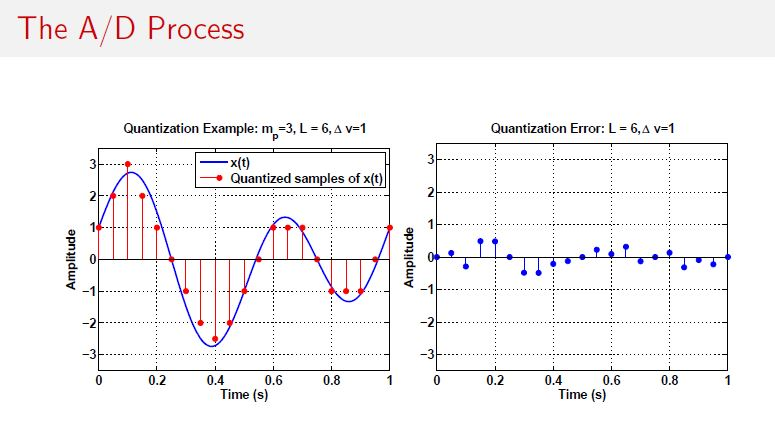
\includegraphics[width = 0.7\textwidth, frame]{Figures/Sampling/quantizaiton_example}
\caption{Quantization Example}
\label{fig:Sampling:quantizaiton_example}
\end{figure}


\begin{itemize}

\item In A/D process, first we sample the signal then we round up the value to a defined level

\item The parameters of the quantization (rounding) are:

	\begin{enumerate}
	\item The number of levels $L$: here we have 6 levels
	
	\item The step size between each level $\delta v$
	
	\item The peak value of the signal $m_p$
	\end{enumerate}


\newpage
\item Now \tbi{rounding introduce errors}, known here as \tbi{quantization error}

	\begin{itemize}
	\item If we want to decrease the quantization error, we need to increase the number of levels $L$ as \autoref{fig:Sampling:quantizaiton_example_2}
	
	\item However we need to allocate more bits to represents all of these levels (trade off)
	
	
	\begin{figure}[h]
\centering
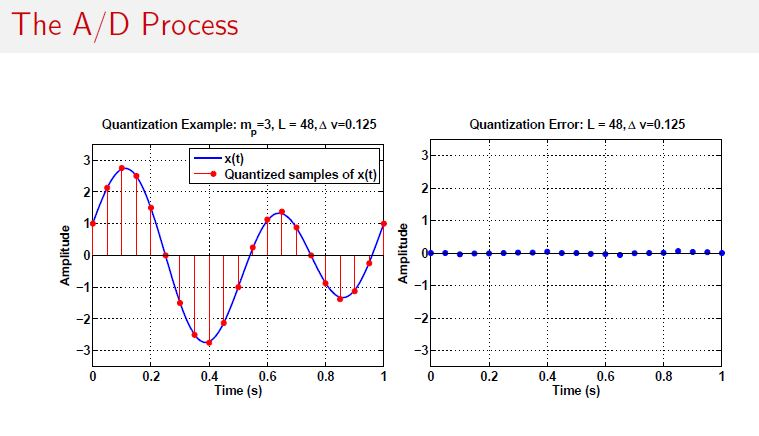
\includegraphics[width = 0.7\textwidth, frame]{Figures/Sampling/quantizaiton_example_2}
\caption{Increasing number of levels $L$ to decrease quantization error}
\label{fig:Sampling:quantizaiton_example_2}
\end{figure}
	
	\end{itemize}

\end{itemize}


\underline{Qunatization Formula:}

\begin{equation}
x_{\text{qunatized}} \, = \, \text{round} \left(\, \displaystyle\frac{x}{\text{step size}}\, \right) \, \times \, \text{step size}
\end{equation}


\newpage
\subsection{Dynamic Range of an Ideal ADC}

\begin{figure}[h]
\centering
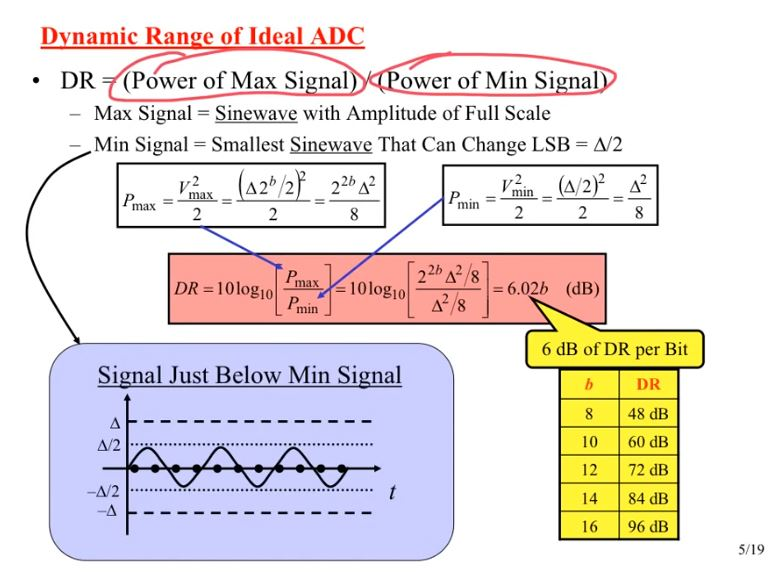
\includegraphics[width = 0.7\textwidth, frame]{Figures/Sampling/dynamic_range_ideal_adc}
\caption{Dynamic Range of an Ideal ADC}
\label{fig:Sampling:dynamic_range_ideal_adc}
\end{figure}


\subsection{Error Analysis of the Quantization Error}

Since qunantization error is unpredictable, we use statistical analysis and probability laws to describe the error.


\begin{equation}
\begin{array}{rcl}
e_q[k] \, &=& \, x[k] \, - \, x_q[k] \\\\
\displaystyle\frac{- \text{step}}{2} &\leq \, e_q[k] \, &\leq \, \displaystyle\frac{+ \text{step}}{2} \\ \\
\text{step} \, &=& \, \displaystyle\frac{\text{Range}}{\text{nb of Levels}} \\ \\
&=& \, \displaystyle\frac{\text{Range}}{2^{\left(\,\text{nb of bits + 1} \, \right)}  }
\end{array}
\end{equation}


\newpage
Error Analysis is shown in \autoref{fig:Sampling:quantizaiton_error_analysis}.

\begin{figure}[h]
\centering
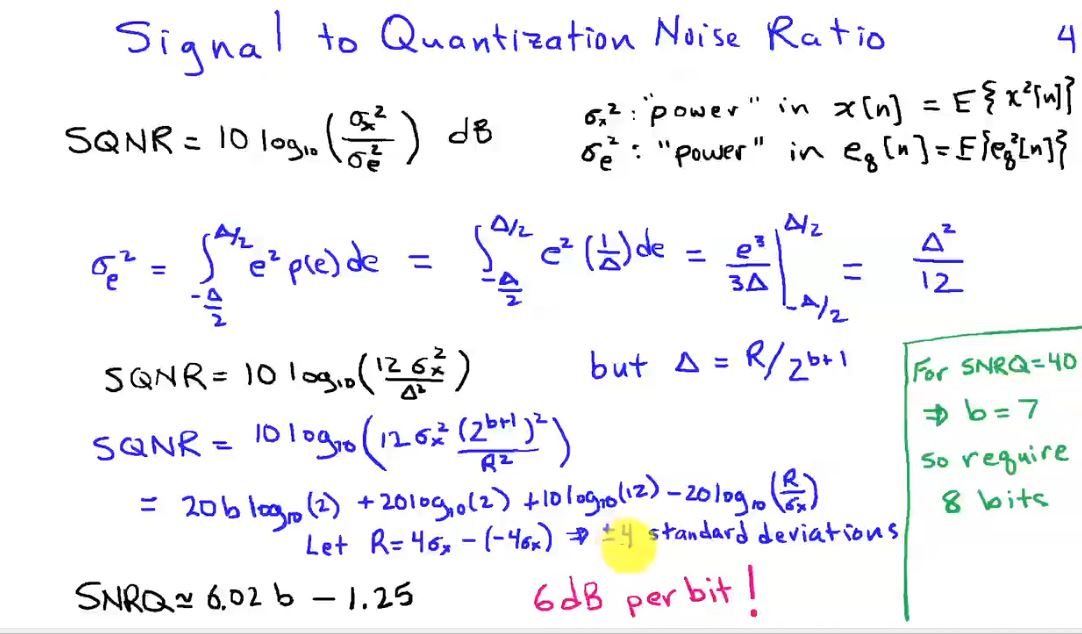
\includegraphics[width = 0.7\textwidth, frame]{Figures/Sampling/quantizaiton_error_analysis}
\caption{Qunatization Error Analysis}
\label{fig:Sampling:quantizaiton_error_analysis}
\end{figure}

\begin{itemize}

\item 

\begin{equation}
\begin{array}{rcl}
\text{SNQR} 	\, &=& \, 10 \, \text{log}_{10} \left(\, \displaystyle\frac{\sigma_x^2}{\sigma_e^2} \, \right) \\ \\
			& \approx & \, 6.02 \, - \, 1.25 \text{ dB/bit}		
\end{array}
\end{equation}


\item The analysis done is under particular assumptions for this statistical analysis:

	\begin{enumerate}
	\item $e_q[k]$ is a stationary random process with a uniform continuous distribution 
	
	\item $e_q[k]$ values are uncorrelated
	
	\item $e_q[k]$ and $x[k]$ are independent 
	\end{enumerate}

\end{itemize}


\newpage
In \autoref{fig:Sampling:quantizaiton_error_example}, we have an example of quantized and non-quantized sin.



\begin{figure}[h]
\centering
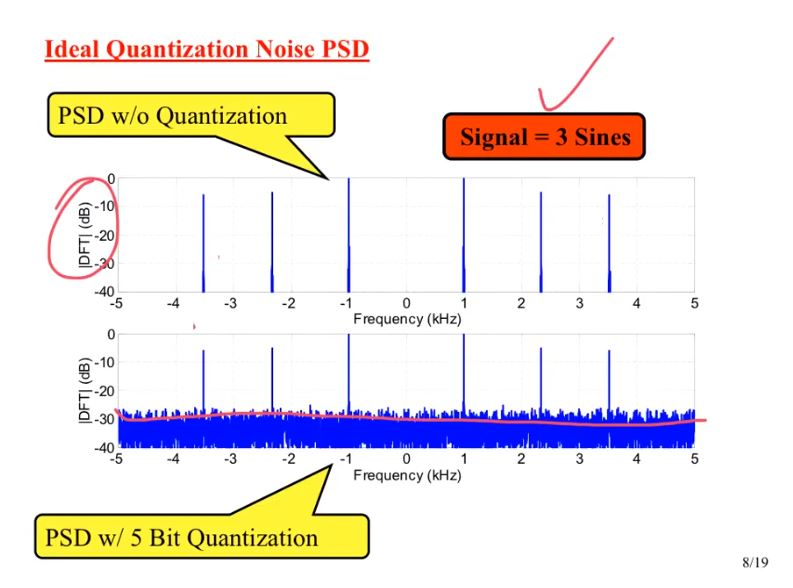
\includegraphics[width = 0.7\textwidth, frame]{Figures/Sampling/quantizaiton_error_example}
\caption{Qunatization Error Example}
\label{fig:Sampling:quantizaiton_error_example}
\end{figure}


\begin{itemize}

\item We can see that the power sepctral density in the quantized part is flat over all the frequency ranges


\item If we use fewer bit in the quantization process, the noise floor will get up

\end{itemize}


\newpage
\underline{SNQR for Full Scale Sine wave:}\\

\begin{figure}[h]
\centering
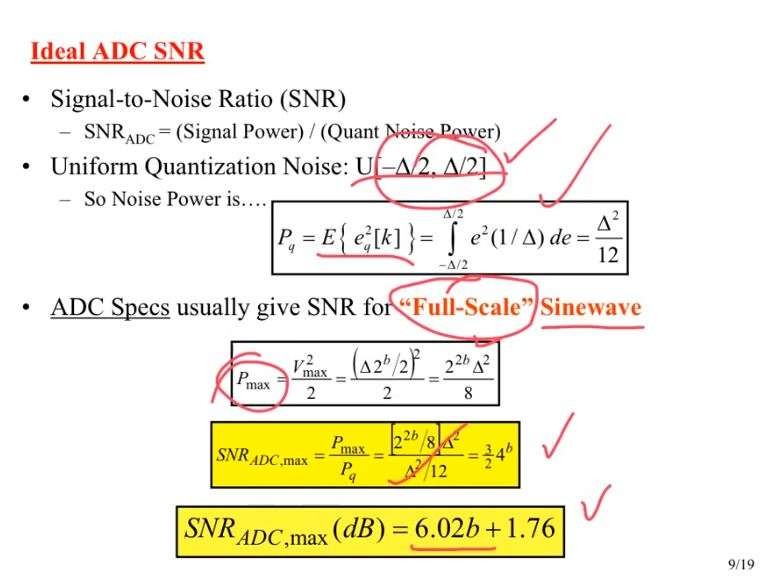
\includegraphics[width = 0.7\textwidth, frame]{Figures/Sampling/snr_full_sin_wave}
\caption{SNR for full sin wave}
\label{fig:Sampling:snr_full_sin_wave}
\end{figure}


\begin{itemize}
\item The SNQR in \autoref{fig:Sampling:snr_full_sin_wave} is a little bit optimistic because we are assuming a full range for the sin wave
\end{itemize}

We can generalize more the SNQR as in \autoref{fig:Sampling:snr_peak_factor}, where use the idea of peak factor to see the exact SNQR.


\newpage
\begin{figure}[h]
\centering
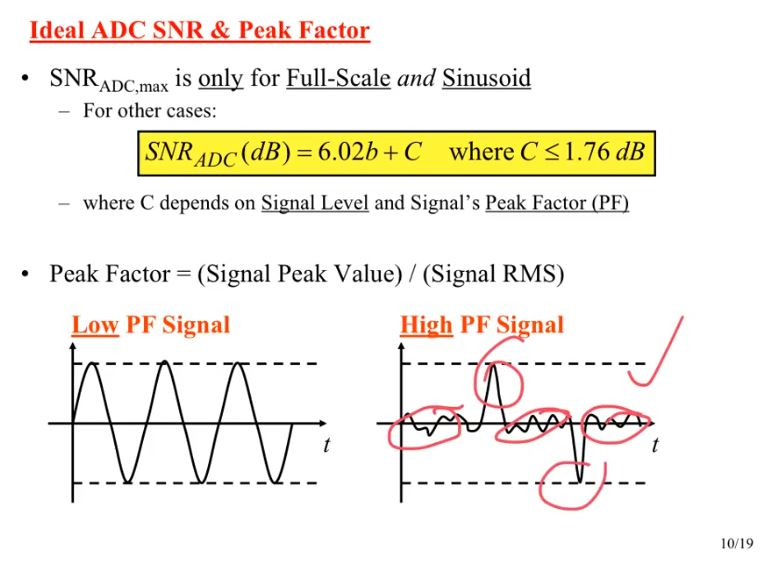
\includegraphics[width = 0.7\textwidth, frame]{Figures/Sampling/snr_peak_factor}
\caption{SNR and peak factor}
\label{fig:Sampling:snr_peak_factor}
\end{figure}

\autoref{fig:Sampling:snr_peak_factor_relation} shows the relation of SNQR and peak factor in dB.


\begin{figure}[h]
\centering
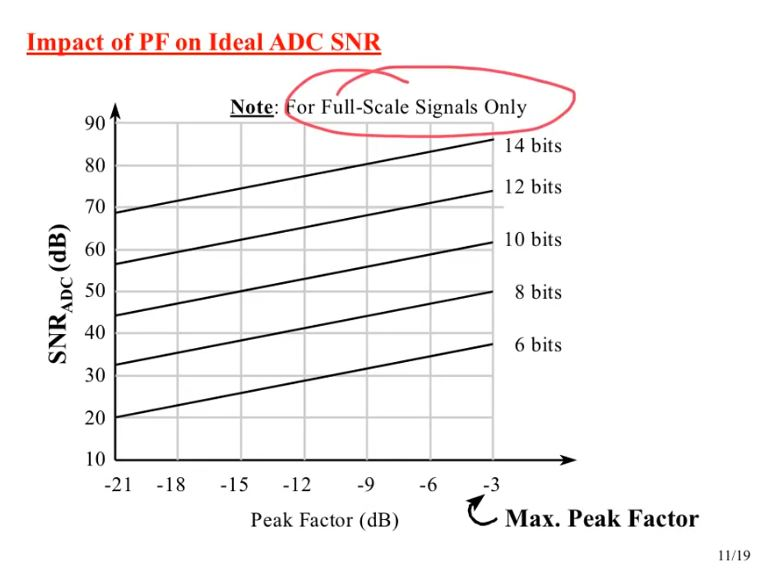
\includegraphics[width = 0.7\textwidth, frame]{Figures/Sampling/snr_peak_factor_relation}
\caption{SNR and peak factor relation}
\label{fig:Sampling:snr_peak_factor_relation}
\end{figure}

\begin{itemize}
\item The more the signal is peaky for a fixed number of bits, the more SNQR is low
\end{itemize}


\subsection{More Source of Errors}

\autoref{fig:Sampling:more_error} shows more sources of errors we can get

\begin{figure}[h]
\centering
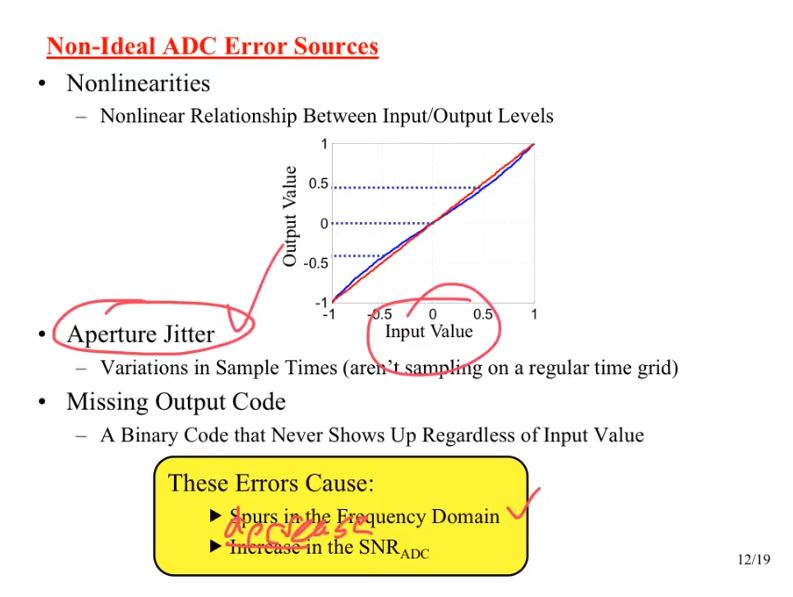
\includegraphics[width = 0.7\textwidth, frame]{Figures/Sampling/more_error}
\caption{SNR and peak factor relation}
\label{fig:Sampling:more_error}
\end{figure}

\begin{itemize}

\item Jitter: comes from clock circuitry we use to do the sampling


\item These errors also shows decrease in the SNQR

\end{itemize}

\autoref{fig:Sampling:spurse} shows how the spruse comes into the amplitude spectrum plots in addition to the noise floor.

\begin{figure}[h]
\centering
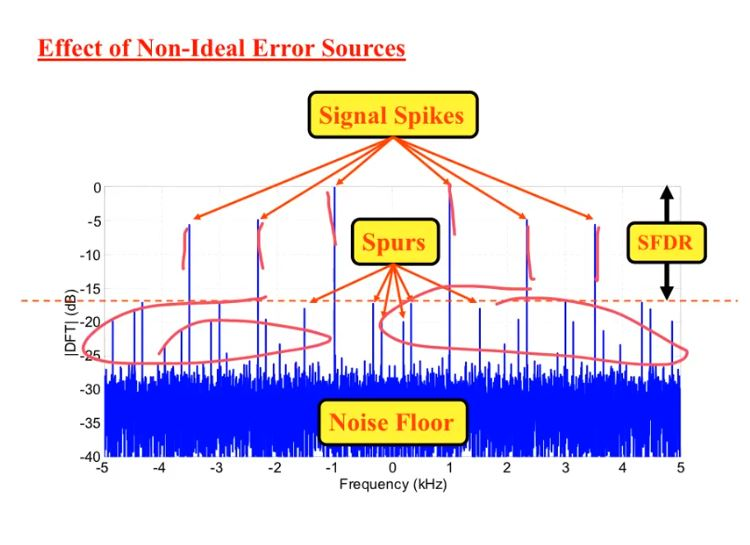
\includegraphics[width = 0.7\textwidth, frame]{Figures/Sampling/spurse}
\caption{Spurse Errors in the Spectrum}
\label{fig:Sampling:spurse}
\end{figure}

\begin{itemize}
\item SFDR set the distance between the actual signals and the spurse
\end{itemize}


\subsection{Specs for ADC}

\begin{figure}[h]
\centering
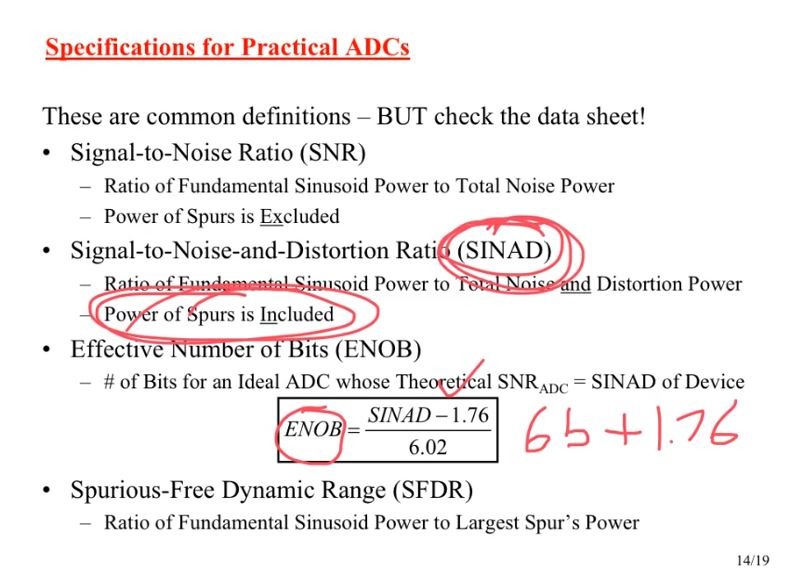
\includegraphics[width = 0.7\textwidth, frame]{Figures/Sampling/ADC_Specs}
\caption{Most common specfication on ADC}
\label{fig:Sampling:ADC_Specs}
\end{figure}

\begin{itemize}

\item ENOB: take into consideration the actual number of bits due SINAD (spurse errors)

	\begin{itemize}
	\item It is the algebraic solution of $\text{SINAD} \, = \, 6 \, \text{bits} \, + \, 1.76$
	
	\item Due to hardware imperfections (spurse), in theory we could have 8 bits, but in reality it may comes down in to 6 bits
	\end{itemize}

\end{itemize}



\newpage
\section{Oversampling and $\Sigma-\Delta$ Converter}

We have seen that oversampling have several advantages. Now let's relate the oversampling to the SNQR.



\begin{itemize}

\item Since we are sampling much higher than the signal bandwidth, we can assume that the signal bandwidth is small compared to $\displaystyle\frac{F_s}{2}$, and the spectrum reside in a small region of the interval $\left[\, \displaystyle\frac{- F_s}{2} \, ; \, \displaystyle\frac{+ F_s}{2} \right] $


\item So we have less noise in the signal spectrum $\rightarrow$ SNQR improve


\item So also ENOB improves

	\begin{itemize}
	\item However at the cost of a higher $F_s$
	\end{itemize}

\item But this is an inefficient trade-off: because we obtain 1 bit per 6 dB

	\begin{itemize}
	\item Computation shown in \autoref{fig:Sampling:oversampling_SNQR_relation}
	
	\begin{figure}[h]
\centering
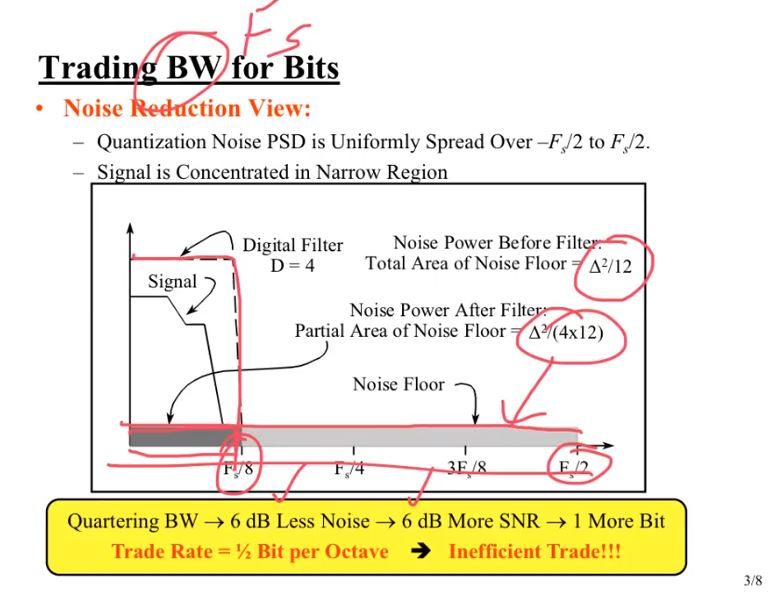
\includegraphics[width = 0.7\textwidth, frame]{Figures/Sampling/oversampling_SNQR_relation}
\caption{Oversampling and SNQR relation}
\label{fig:Sampling:oversampling_SNQR_relation}
\end{figure}	

	\item The noise power is the area under the curve then we divide powers
	
	\end{itemize}

\item So engineers start to search for a better trade-off

\item The idea of $\Sigma-\Delta$ converter: don't touch the signal but push the noise outside the signal spectrum

\newpage
\item Intuition and results are shown in \autoref{fig:Sampling:sigma_delta_noise_shaping}.

	\begin{figure}[h]
\centering
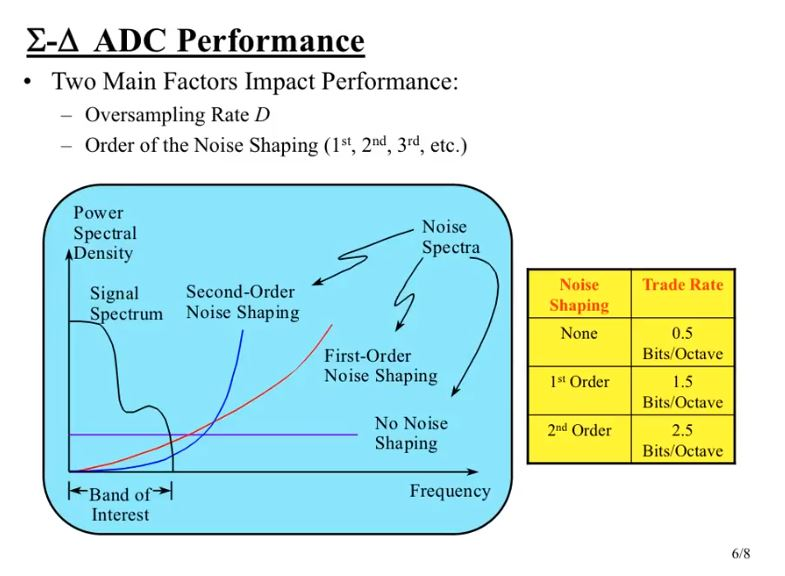
\includegraphics[width = 0.7\textwidth, frame]{Figures/Sampling/sigma_delta_noise_shaping}
\caption{Noise shaping effect}
\label{fig:Sampling:sigma_delta_noise_shaping}
\end{figure}	

	\begin{itemize}
	\item The more we increase the order of noise shaping, the area of the noise decrease and hence SNQR and ENOB increase for the \tbi{band of interest}
	\end{itemize}


\end{itemize}







